\documentclass[a4paper,oneside,11pt,table,xcdraw,normalem]{memoir}

\usepackage[utf8]{inputenc} % input encoding
\usepackage[T1]{fontenc} % font encoding
\usepackage{svg}
\usepackage{graphicx} %to include images/graphics
\usepackage{amsmath,amssymb} %better math type setting
\usepackage{listings} %for source code snippets
\usepackage{textcomp} %for upquote
\usepackage{xcolor} % nice colors (for source code)
\usepackage{amsmath}
\usepackage[table,xcdraw]{xcolor}
\usepackage[normalem]{ulem}
\usepackage{tabularx}

\renewcommand{\ttdefault}{pcr} % nicer font for source code

% an example configuration of the 'listings' package
\lstset{basicstyle=\ttfamily, 
        keywordstyle=\color{purple}\ttfamily,
        commentstyle=\color{gray}\ttfamily,
        stringstyle=\color{orange}\ttfamily,
        captionpos=b,
        float=tb,
        upquote=true,
}

\chapterstyle{tandh} % configuration of the 'memoir' class

%
% The actual document starts here
%
\begin{document}

\begin{titlingpage}
\thispagestyle{empty}

\centering
  \vspace*{6.5em}

  \textsc{\textbf{\huge
    % 
    % Insert your title here
    %
      SPARQL Visualisation Tool
  }}

  \vspace{4.5em}

  \textsc{\Large
    \setlength{\tabcolsep}{12pt}
    \begin{tabular}[h]{lr}
    % 
    % Insert your names and exam numbers here
    %
      Andreas Timm Adriansen        &  anadr18
      \\[.4\onelineskip]
      Andreas Vinggaard Frederiksen    &  afred18
    \end{tabular}
  }

  \vspace{5em}
  \large
  % 
  % Adjust the type of thesis and education here
  % 
  % Bachelor Project in Software Technology
  Bachelor Project in Software Engineering
  % Masters Project in Software Engineering

  \normalsize
  \vspace{2em}
  %
  % Change the date here
  %
  June 2021


  \vspace{12.5em}
  
\includegraphics[width=.5\textwidth]{figures/sdu_logo}
  
  \vspace{3em}
  The Maersk Mc-Kinney Moeller Institute

  \medskip
  University of Southern Denmark

\end{titlingpage}


\cleardoublepage

\frontmatter

% abstract / resume
\begin{abstract}
  Many companies are struggling to combine Java and Machine Learning\dots   
\end{abstract}


\cleardoublepage

\tableofcontents

\mainmatter

%
% We have one file per chapter:
%

% Introduction chapter in 'chap-introduction.tex'
\chapter{Introduction}
\label{chap:introduction}

{\color{red}missing\\}

\section{Context}

SPARQL is a query language, used for querying RDF data models. RDF is a set of specifications that started being used in web resources\cite{W3SchoolsXMLRDF} but now it is more used for Industry4.0 and IoT, it is most commonly stored in .TTL files. RDF is a way of expressing the notion of a triple store, and is intended for machine consumption. Such triples consist of a subject (like a person or something similar), a predicate (defining a relationship), and an object (what the relationship is towards). For instance “Person1 isCalled ‘Andreas’” defines that the subject Person1 has an isCalled relationship to the object ‘Andreas’. In other words; Person1 is called Andreas.
\\\\
RDF is a promising way of modeling data, but SPARQL is foreign to most developers and thus represents a barrier. In this project we seek to make it easier to learn SPARQL.


\section{Problem}
How can we develop a visualiser for writing and understanding SPARQL queries as a new user?
\\\\
That is to say,
\begin{enumerate}
    \item Which visual elements are important for promoting the understanding of the SPARQL query and its syntax?
    \item How would the user interact with the visualisation in such a system, and how is the translation, parsing, done between the visualisation tool and the SPARQL query to avoid problems such as SPARQL injection?
    \item How can we make it possible for the user to save and share their visualisation? 
    \item And lastly, is there a limitation to how many inputs such a visualisation can take before it becomes unresponsive?
\end{enumerate}



\section{Related work}
\subsection{Nitelight}
In a paper by Alistair Russel, Paul R. Smart, Dave Braines, and Nigel R. Shadbolt\cite{Nitelight}, the graphical tool for semantic query construction Nitelight is discussed. Nitelight breaks down SPARQL queries  by utilizing the nature of RDF triple patterns to create visualisations. 
\begin{figure}[h]
    \centering
  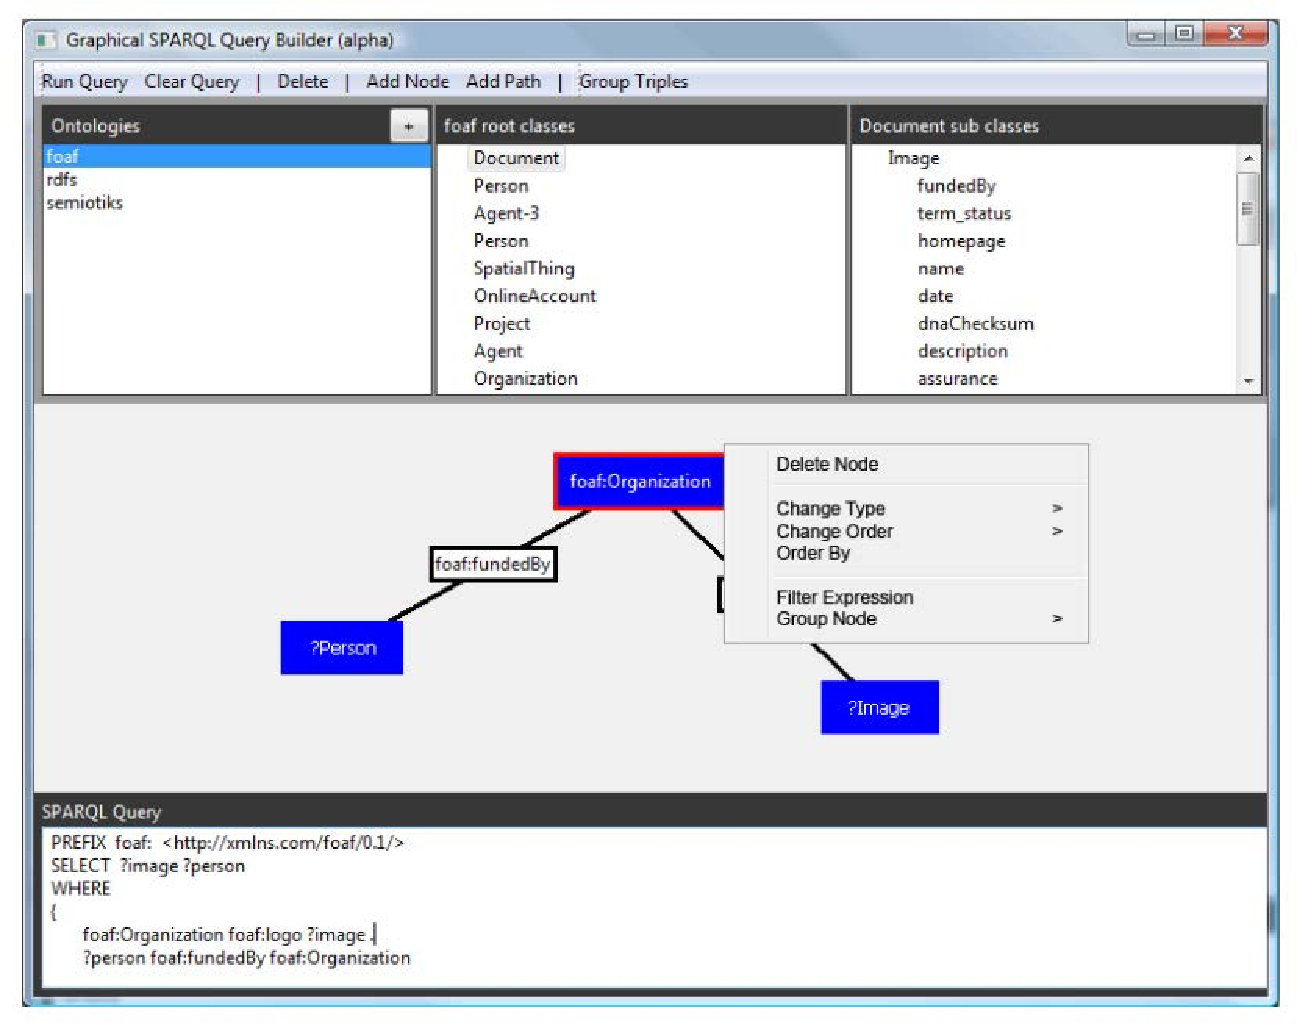
\includegraphics[width=.9\linewidth]{NitelightFigure1.pdf}
  \caption{An overview of the Nitelight user interface\cite{Nitelight}}
  \label{fig:NitelightUI}
\end{figure}
\\
Figure \ref{fig:NitelightUI} is an image of Nitelight in action. Nitelight is developed as a Java application and has some different tools to use. In the top it has basic commands such as running the query and adding new nodes. Below is the ontology browser, which can be used for the user to look through the different ontologies and what they consist of. Under the ontology browser is the node view, which is the main part of Nitelight. Here the nodes are set up in such a way that shows their relation to each other and this all results in the SPARQL query in the bottom. This text view is the result of the visual query and is read only.
\\\\
To elaborate on how the node view represents the finished query, use figure \ref{fig:NitelightBreakDown} for reference. Here it is shown that the query deals with three parts, the bound variable, the unbound variable and the literal predicate. The unbound variable points to the literal predicate, which then points to the bound variable. An example of this can also be seen in figure a, where a person (the bound variable) is funded by (the literal predicate) an organisation (unbound variable).

\begin{figure}[h]
    \centering
  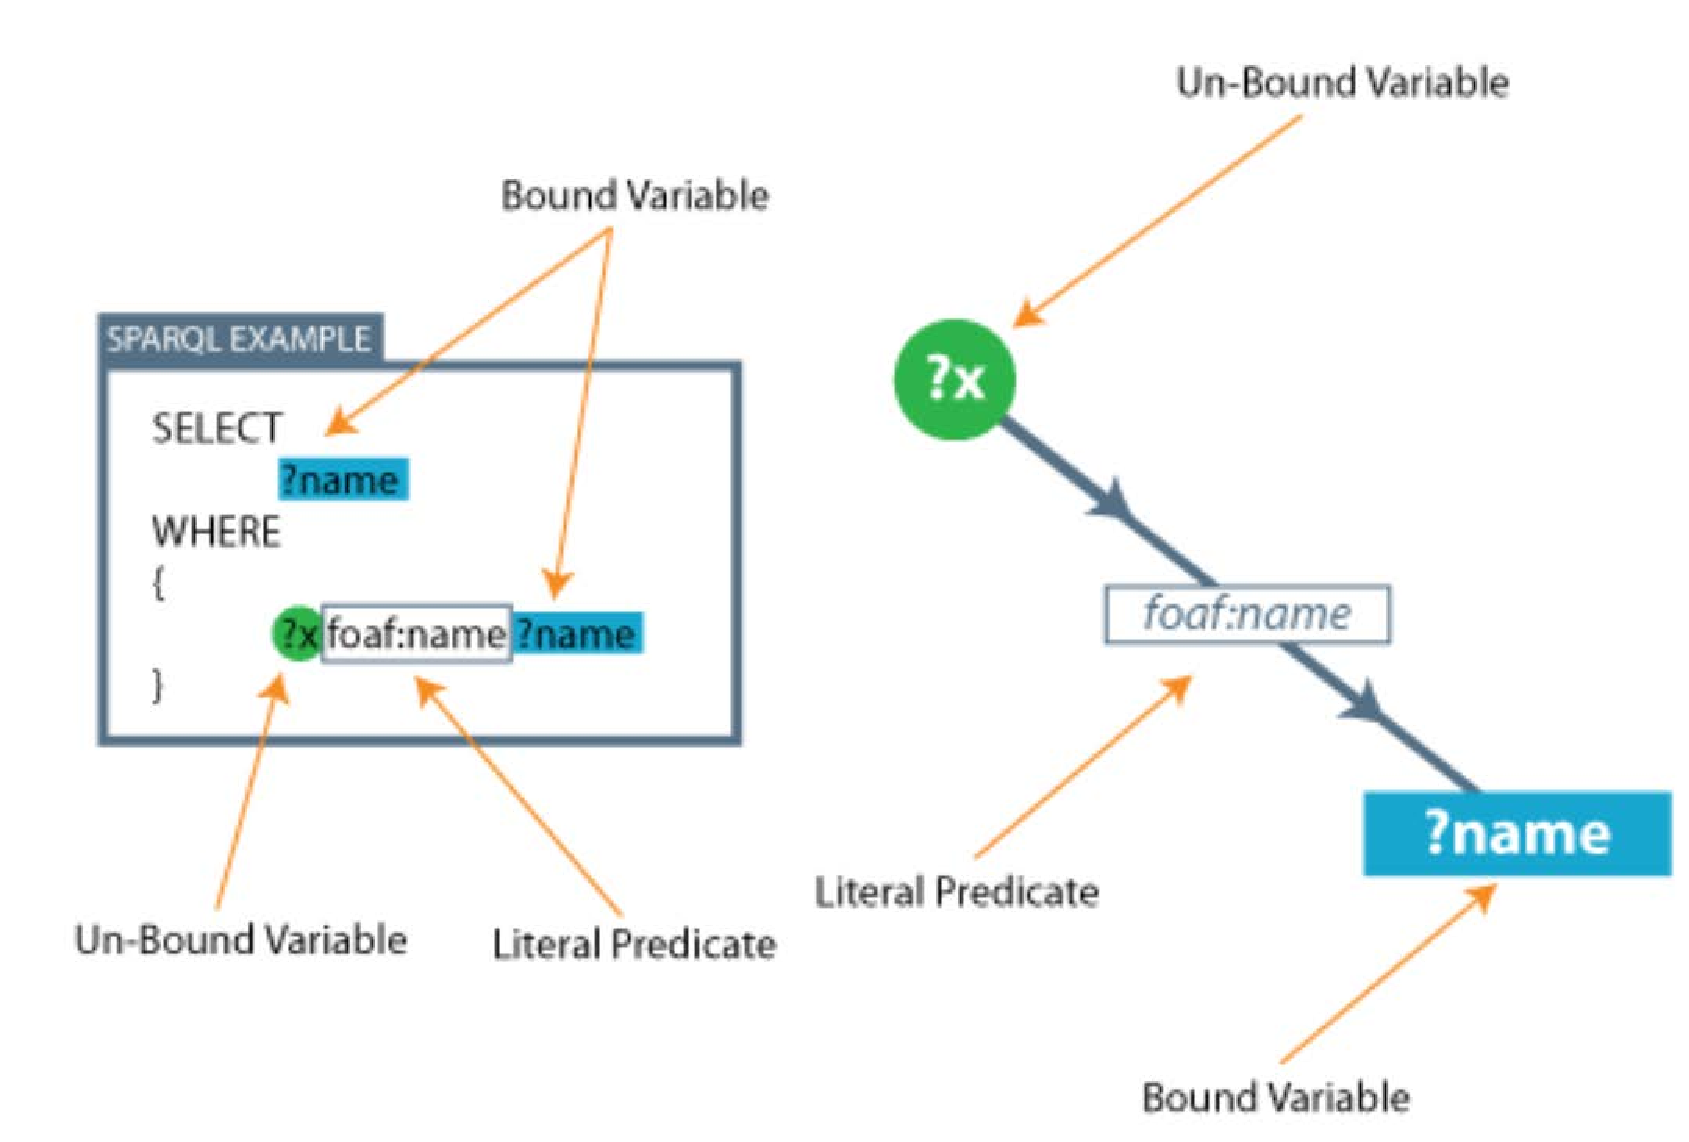
\includegraphics[width=.9\linewidth]{NitelightFigure2.pdf}
  \caption{Breaking down SPARQL queries to visualization\cite{Nitelight}}
  \label{fig:NitelightBreakDown}
\end{figure}

\subsection{QueryVOWL}
QueryVOWL is a visual query language to help users develop SPARQL queries\cite{QueryVOWL}, similarly to Nitelight. It is however developed as a webcomponent using HTML, CSS, JavaScript and SVG. It has three views, the main visual view, the sidebar for additional options and a result list containing the SPARQL query. The main view implements a drag and drop interface, which results in a completed SPARQL query without the need for the user to know perfect syntax. It can take any RDF dataset containing SPARQL endpoints.

\subsection{SPARQL-visualizer: A Communication Tool for Collaborative Ontology Engineering Processes}
This is a visualisation of the query result\cite{MadsHoltenSPARQL} and not the query itself. Therefore it could seem less relevant, however the way the graphical elements are implemented is something that can be used as inspiration. This leads to the library D3.js, a graphics library in JavaScript. The paper references (https://github.com/Rathachai/d3rdf) as a way to create a force layout of D3.js to visualize the expression "subject–predicate–object".



\section{Approach}
The solution will consist of a webcomponent, using JavaScript, that has two views for composing SPARQL queries, a textual and a visual. The visual view will be processed through SVG and should come in the form of a spring graph model layout. The user can interact with the visualisation through a drag and drop interface. The visualisation will then affect the textual view by writing the query in text. Likewise, will the visual view be affected by the textual view. Lastly, the visualisation has the option to be saved locally.

\section{Project goals}
The goals for this project are:
\begin{enumerate}
    \item To learn about RDF and SPARQL.
    \item To make a tool for visualising SPARQL queries.
    \item To make it easy to visualise and convert between a graphical and textual view of a SPARQL query.
\end{enumerate}

\section{Report structure}
{\color{red}missing\\}

% Background chapter in 'chap-background.tex'
\chapter{Background}
\label{chap:background}

In this chapter we recall the Java type system and the fundamentals of
machine learning.

\section{The Java Programming Language}

Here is a section on Java.

\section{Machine Learning}

Here is another section.


% ...
\chapter{Requirements}
\label{chap:requirements}

This chapter deals with defining and analysing of requirements for the project. To help determining the requirements, a list of use cases is created. The requirements are split into two categories: functional requirements and non-functional requirements. Using the two tools, MoSCoW  and FURPS , the requirements are then evaluated and prioritized.

\section{Use case}
Before determining the requirements, a list of use cases  is created to better understand what is essential for the user experience. This list can be seen in table \ref{tab:usecases} below.

\begin{table}[h]
\begin{tabularx}{\textwidth}{|l|l|X|X|}
\hline
\rowcolor[HTML]{9B9B9B}
ID   & Use case name      & Pre-Condition                                               & Post-Condition                                                    \\ \hline
\#01 & Add node           & Add node tool is selected                                   & After a successful creation, a node is added to the visualisation \\ \hline
\#02 & Draw arrow         & Draw line tool is selected, two nodes in visualisation      & A line is drawn between two nodes                                 \\\hline
\#03 & Delete nodes       & Nodes are selected                                          & The nodes are deleted from the visualisation                      \\\hline
\#04 & Delete arrows      & Arrows are selected                                         & The arrows are deleted from the visualisation                     \\\hline
\#05 & Write queries      & Text field is selected                                      & The text field is updated                                         \\\hline
\#06 & Save visualisation & Visualisation is not empty                                  & The visualisation has been saved locally                          \\\hline
\#07 & Edit node          & The edit tool is selected, a node is in the visualisation   & The node has been altered                                         \\\hline
\#08 & Edit arrow         & The edit tool is selected, an arrow is in the visualisation & The arrow has been altered    \\\hline   
\end{tabularx}
\label{tab:usecases}
\caption{Use cases for the program}
\end{table}

Each use case from table \ref{tab:usecases} is then expanded to include the possible scenarios in a separate table. An example of this is in \ref{tab:drawarrowusecase} which shows the extended version of the “Draw arrow” use case. By expanding the use case like this, the technical aspects of the use case can be described which can help in requirement elicitation and development.

\begin{table}[h]
\begin{tabularx}{\textwidth}{|l|l|X|}
\hline
\rowcolor[HTML]{9B9B9B}
Main Scenarios & Serial no. & Steps                                                                                          \\ \hline
Actors/Users   & \#01       & Click on two nodes                                                                             \\ \hline
               & \#02       & A popup occurs for arrow creation                                                              \\ \hline
               & \#03a      & Input name and press submit                                                                    \\ \hline
               & \#04a      & \begin{tabular}{@{}l@{}}An arrow is created\\ Close popup\end{tabular}                \\ \hline
               & \#03b      & Close popup                                                                                    \\ \hline
Extensions     & \#01       & \begin{tabular}{@{}l@{}}Nodes are already connected\\     Show error message\end{tabular} \\ \hline
               & \#03a      & \begin{tabular}{@{}l@{}}Name is not eligible\\    Show error message\end{tabular} \\ \hline                   
\end{tabularx}
\label{tab:drawarrowusecase}
\caption{Expanded use case for "\#02 Draw arrow"}
\end{table}

\section{Functional requirements}
Using the list of use cases, a set of functional requirements can be determined. The functional requirements are then prioritized using the MoSCoW method. This method deals with four different types of requirement prioritization: Must have, should have, could have, and will not have. The functional requirements can be seen in table \ref{tab:funcrequirements}.

\begin{table}[h]
\centering
\begin{tabular}{|l|l|l|}
\hline
\rowcolor[HTML]{9B9B9B}
ID  & Title                       & MoSCoW \\ \hline
\#01 & Node creation               & M      \\ \hline
\#02 & Arrow creation              & M      \\ \hline
\#03 & Writeable query             & M      \\ \hline
\#04 & Example of query            & C      \\ \hline
\#05 & Editable nodes              & S      \\ \hline
\#06 & Editable arrow              & S      \\ \hline
\#07 & Query and node highlighting & S      \\ \hline
\#08 & Visual and textual updating & M      \\ \hline
\#09 & Textual input parsing       & M      \\ \hline
\#10 & Parsing error handling      & S      \\ \hline
\#11 & Saving locally              & S      \\ \hline
\#12 & Uploading saves             & C      \\ \hline
\#13 & Multiple query types        & S      \\ \hline
\end{tabular}
\label{tab:funcrequirements}
\caption{Functional requirements}
\end{table}

Must have requirements are critical functionality. This means that without these, the program would be non-functional, or it would be impossible to implement other functionalities. An example of this is the node creation requirement. Without this functionality, there is not really a lot of program left. It would be impossible to work together with the textual view, saving the visualisation, add arrows, etc. Must have requirements are therefore often also reflected by the most important use cases.

\section{Non-functional requirements}
The non-functional requirements do not necessarily reflect the use cases but are requirements that influence the experience of the system. In this section, non-functional requirements are set through the process of a FURPS analysis. FURPS stands for: Functionality, Usability, Reliability, Performance, and Supportability. Functionality will be disregarded as this belongs to the functional requirements.

\subsection{Usability}
The target user for the application has no experience with RDF and SPARQL. This implies the application should focus on beginner level SPARQL and ease the user into writing queries. The application should be easy to figure out in the first couple of minutes. To help understand the concepts within SPARQL, the use of highlighting could be implemented into the system. This means that different attributes of the query could be highlighted consistently across the application making it easier to connect the visualisation to the written query. The user interface does not need to be visually pleasing, as the functionality is prime, but it should be consistent and therefore intuitive to use.

\subsection{Reliability}
The software needs to be working without any critical failures in the code. The application shall not store any user data, but it could be useful to cache the visualisation on updates, to help recoverability in case of shut-down failure. The application will not focus on loading times for different devices.

\subsection{Performance}
Once loaded, the application should run smoothly, preferably even on low end computers. There should not be any noticeable delay between actions. Actions should be done within 100 milliseconds of a user input, and if not, some sort of indication that the action is being processed should be shown.

\subsection{Supportability}
The application must be maintainable and open to future alterations. The application shall work as a web component and should therefore be easy to add to a webpage. The application will not be expected to support other devices than PC’s.

% Analysis and Design chapter in 'chap-analysis-and-design.tex'
\chapter{Analysis and Design}
\label{chap:analysis-and-design}


\bigskip

\dots We summarize something in Table~\ref{tab:java-advantages}.

\begin{table}[tb] % placement: h for here, t for top, b for bottom
  \centering
  \begin{tabular}{l c}  % two columns: l for left, c for center, r for right
    Feature  & Benefit
 \\\hline
    Objects  & State encapsulation
 \\
    Generics & Code reuse
  \end{tabular}
  \caption{Advantages of Java}
  \label{tab:java-advantages}
\end{table}

\bigskip

\noindent
LaTeX indents a new paragraph unless you specify \lstinline{\noindent}.

\bigskip

We can also refer to Figure~\ref{fig:firefox-js-console}.

\begin{figure}[tb] % placement: h for here, t for top, b for bottom
  \centering
  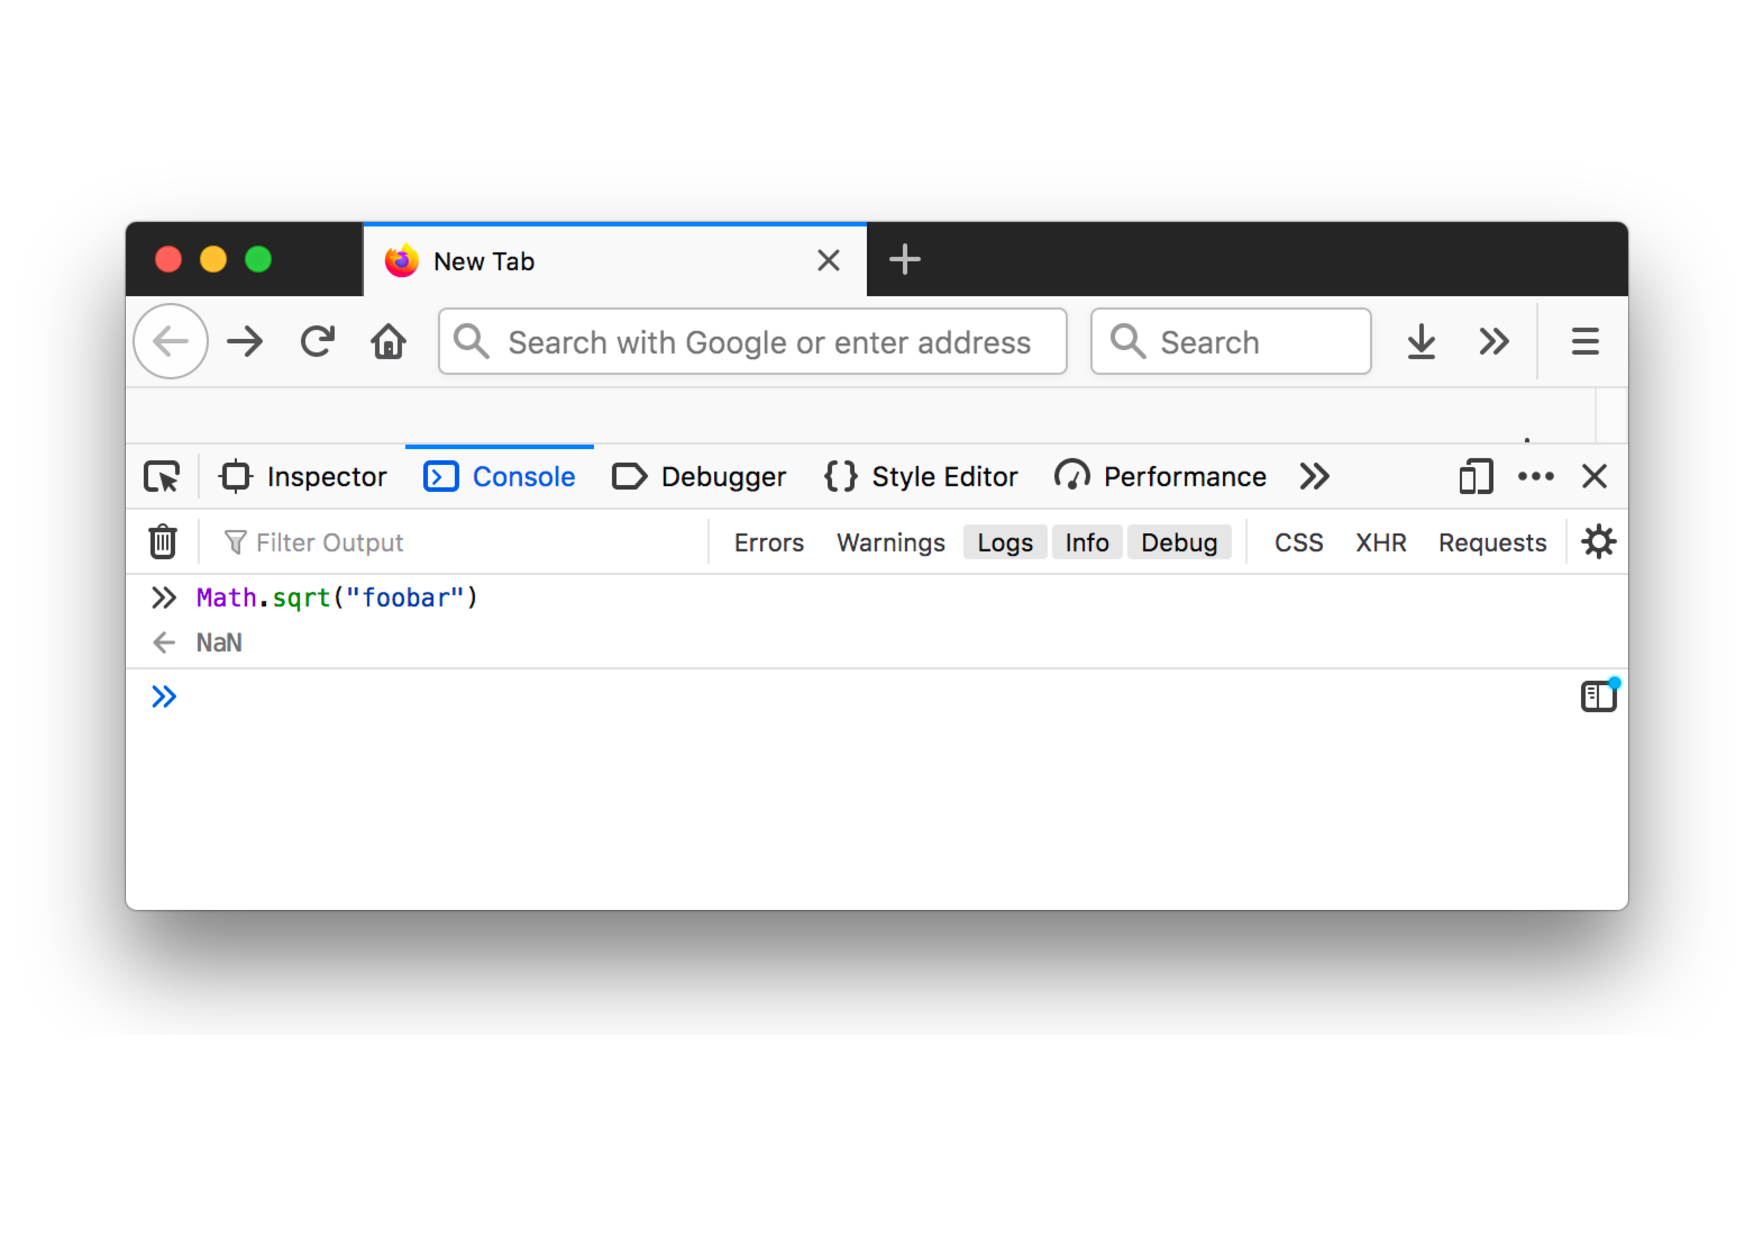
\includegraphics[width=.9\linewidth]{firefox-js-console}
  \caption{The JavaScript console in Firefox }
  \label{fig:firefox-js-console}
\end{figure}


% Implementation chapter in 'chap-implementation.tex'
\chapter{Implementation}
\label{chap:implementation}

We can refer to Chapter~\ref{chap:analysis-and-design} for something.

\bigskip

Here is an example formula to compute a sum:
%
\begin{align*}
  \sum_{i=1}^{n} = \frac{n (n+1)}{2}
\end{align*}

Math can also be included inline $a (b + c) = a b + a c$ in a sentence.

\bigskip
We refer to Listing~\ref{lst:sum} for the Java implementation.\\ % force new line
Code snippets like \lstinline{System.out.println} can also be given inside a sentence.

\begin{lstlisting}[language=java,caption={Our sum implementation},float=tb,label=lst:sum]
  class Sum {
    public static void main(String[] args) {
      int n = 5;   // the input
      int sum = n * (n+1);
      System.out.println("The sum is: " + sum);
    }
  }
\end{lstlisting}

\bigskip

Finally we can refer to some material in Appendix~\ref{appendix:api-doc}. 


% Conclusion chapter in 'chap-conclusion.tex'
\chapter{Conclusion}
\label{chap:conclusion}

Overall our project was a success.


\appendix

test

% Appendix chapter in 'chap-appendix.tex'
\chapter{Appendix}
\label{appendix:api-doc}

We include here the API documentation for our library.


\bibliographystyle{IEEEtran}
\bibliography{mybibliography}

\newpage

\listoffigures

\newpage

\listoftables

\newpage

\begin{figure}
    \centering
    \includesvg[width=.9\linewidth]{UI_idea_1.svg}
    \caption{Caption}
    \label{fig:my_label}
\end{figure}

\begin{figure}
    \centering
    \includesvg[width=.9\linewidth]{UI_idea_2.svg}
    \caption{Caption}
    \label{fig:my_label}
\end{figure}

\begin{figure}
    \centering
    \includesvg[width=.9\linewidth]{UI_idea_3.svg}
    \caption{Caption}
    \label{fig:my_label}
\end{figure}


\end{document}
